\documentclass[english]{tktltiki}
\usepackage[pdftex]{graphicx}
\usepackage{subfigure}
\usepackage{url}
\usepackage{enumerate}
\usepackage{amsmath}
\usepackage{hyperref}
\begin{document}
\onehalfspacing

\title{Location Awareness - Week 3}
\author{P�ter Ivanics}
\date{\today}

\maketitle

\numberofpagesinformation{\numberofpages\ pages + \numberofappendixpages\ appendices}
\keywords{}

\mytableofcontents

\section{Location systems}
	\begin{enumerate}[a)]
		\item Beacon Scan Request is a periodic broadcast request generated by mobile devices based on Bluetooth Low Energy or WiFi signals. It allows to identify being in the proximity of beacons, which may store valuable information for the user. On top of that, since beacons can approximate the distance of the devices based on the broadcast signal strength, positioning algorithms may be applied to determine the relative position of the users. 
	\item Range and Pseudorange (biased range) are terms used in Global Positioning System (GPS), which refer to the distance between a satellite and a device calculated based on the satellite's broadcast message.
	
	The range is estimated based on the orbital position and the system time of the satellite, which is embedded in its broadcast message. The challenge is that the calculations may not precise, because the receiver's and the satellite clock times are typically not synchronized.
	
	 Pseudorange estimates the position based on the receiver's clock offset as an unknown variable. In order to determine one's position correctly, the pseudorange for 4 different satellites has to be calculated at least. As a result, the pseudorange calculation is more precise in comparison to regular range calculations. 
	
	\item Table \ref{positioning-errors} summarizes the accuracy for different percentiles while Figure \ref{positioning-errors-plot} visualizes the errors of the given systems. From this data we can see that System 1 is more accurate on average, as the its mean is only $4.65$ while System 2 has a mean error of $5.39$. Furthermore, System 1 is more consistent as it produces less errors for all percentiles. 
 	
		\begin{table}[]
		\centering
		\caption{The accuracy of the given systems in the $positioningErrors.csv$. }
		\label{positioning-errors}
		\begin{tabular}{lll}
			& System 1 & System 2 \\ \hline
			Mean error & 4.654359 & 5.390046 \\
			100-percentile & 18.935   & 28.837   \\
			99-percentile  & 13.568   & 15.442   \\
			95-percentile  & 11.067   & 12.817   \\
			50-percentile  & 4.0117   & 4.6446
		\end{tabular}
		\end{table}
				
			\begin{figure}[h] 
			\begin{center}
				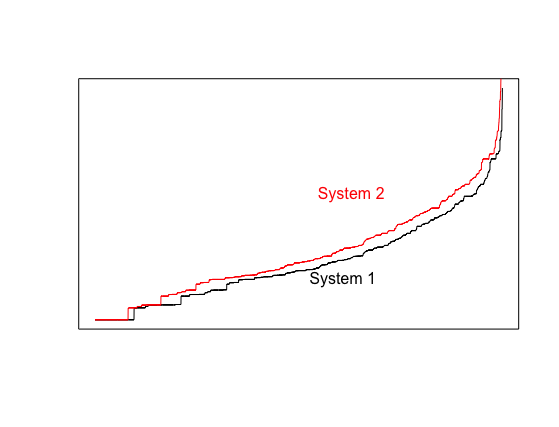
\includegraphics[width=0.75\textwidth]{images/positioningErrorsCDF.png}
				\caption{The CDF plot of the positioning errors.}
				\label{positioning-errors-plot}
			\end{center}
		\end{figure}		
		
	\end{enumerate}
\section{GPS}
	The attached $gps.R$ script was developed to calculate the matrix and Delution of Precision (DOP) values. 
	\begin{enumerate}[a)]
		\item The DOP matrix (as noted by A in the lecture slide) was calculated using the given receiver coordinates $(2884008, 1341225, 5509960)$ and the last three satellite coordinates [$(1822872, 1385835, 6811632), (3564658, 1023739, 6111277)$ and \\ $(2298939, 2257674, 6224440)$]. The following matrix was calculated as a result:
			
		\[
		A=
		\begin{bmatrix}
			-0.5348531 & -0.38981724 & 0.7496497 &  -1 \\
			-0.6316342 & 0.02655381 & 0.7748117 &  -1 \\
			0.7074523 &  -0.32998782 & 0.6249954 &  -1 \\
			-0.4496985 & 0.70440535 & 0.5491670  & -1
		\end{bmatrix}		
		\]	
		 
		\item The calculated DOP values are, as follows: 
				\[
				Q = (A^T * A)^{-1} = 
				\begin{bmatrix}
					1.165599 & 1.033347 & 5.024915 & 2.935933 \\
					1.033347 & 2.813616 & 9.561435 & 5.954195 \\
					5.024915 & 9.561435 & 64.074904 & 40.814138 \\
					2.935933 & 5.954195 & 40.814138 & 26.289674
				\end{bmatrix}	
				\]	
			\begin{eqnarray*}
				HDOP = \sqrt((Q_{11} + Q_{22})) = 1.995 \\
				VDOP = \sqrt(Q_{33}) = 8 \\
				PDOP = \sqrt((Q_{11} + Q_{22} + Q_{33})) = 8.25
			\end{eqnarray*}
		\item The most reliable component of the three above is the horizontal precision (HDOP) as it has the lowest value, while the least reliable component is the Positional precision (3D position, PDOP) as it has the highest value. According to the  \href{https://en.wikipedia.org/wiki/Dilution_of_precision_(navigation)}{\textbf{Wikipedia article on Delution of precision}}, the DOP values above 10 are considered moderately good and are classified as \textit{"Positional measurements could be used for calculations, but the fix quality could still be improved. A more open view of the sky is recommended."}
	\end{enumerate}

\section{Particle Filter}
	The implementation of the particle filter can be found in the attached $particleFilter.R$ file. 
	
	\begin{enumerate}[a)]
		\item The particles' weight values are updated by the $getUpdatedWeight()$ and the values are normalized by the $normalizeWeights()$ function. The results are displayed in Table \ref{derived-new-weights} both before and after normalization.
		
		\item The $needsResampling()$ function returns the response as a boolean if resampling is needed for the actual weights of the particles. As the number of effective particles (inverted squared sum) of the normalized weights in Table \ref{derived-new-weights} equals to $N_{eff}=6.281596$, the threshold of $N_{treshold}=2$ is exceeded and therefore resampling is not needed.
		\item The derived weights before and after normalization are displayed in Table \ref{derived-new-weights2}. As the number of effective particles (inverted squared sum) of the normalized weights in Table \ref{derived-new-weights2} equals to $N_{eff}=1.232329$, the threshold of $N_{treshold}=2$ is not exceeded and therefore resampling is needed.
		
	\begin{table}[]
		\centering
		\caption{The derived new weights for the particles using the given movement model on item a).}
		\label{derived-new-weights}
		\begin{tabular}{lll}
			Weight index & Before normalizing & After normalizing \\ \hline
			1 & 0.003315905 & 0.02596887 \\
			2 & 0.011274076 & 0.08829417 \\
			3 & 0.004839414 & 0.03790041 \\
			4 & 0.025810211 & 0.20213552 \\
			5 & 0.016131382 & 0.12633470 \\
			6 & 0.012600438 & 0.09868172 \\
			7 & 0.001613138 & 0.01263347 \\ 
			8 & 0.020127105 & 0.15762765 \\
			9 & 0.001326362 & 0.01038755 \\
			10 & 0.030649625 & 0.24003593
		\end{tabular}
		
		\caption{The derived new weights for the particles using the given movement model on item c).}
		\label{derived-new-weights2}
		\begin{tabular}{lll}
			Weight index & Before normalizing & After normalizing \\ \hline
			1 & 0.0001 & 0.0001 \\
			2 & 0.0001 & 0.0001 \\
			3 & 0.0003 & 0.0062 \\
			4 & 0.0014 & 0.0329 \\
			5 & 0.0009 & 0.0206 \\
			6 & 0.0001 & 0.0001 \\
			7 & 0.0001 & 0.0021 \\
			8 & 0.0387 & 0.8991 \\
			9 & 0.0001 & 0.0001 \\
			10 & 0.0017 & 0.0391
		\end{tabular}
		\end{table}
	\end{enumerate}
	
\nocite{*}
\bibliographystyle{tktl}
\bibliography{lahteet}

\lastpage

\pagestyle{empty}

\end{document}